\documentclass[../../main.tex]{subfiles}
\begin{document}

{\bf[解]}

\subparagraph{(1)}

\begin{figure}[htb]
  \centering
  \tdplotsetmaincoords{70}{55}
  \begin{tikzpicture}[scale=1.3, >=stealth, every node/.style={font=\small}]
    \begin{scope}[tdplot_main_coords]
      % 座標軸
      \draw[->] (-1.5,0,0) -- (1.5,0,0) node[below left=1pt] {$x$};
      \draw[->] (0,-0.5,0) -- (0,3.2,0) node[right] {$y$};
      \draw[->] (0,0,-0.3) -- (0,0,3.2) node[above] {$z$};

      % 影 S の境界 T（z=0 平面内，中心 (0,√2,0)，半径 √2）
      \draw[dashed] plot[domain=0:360, samples=80, variable=\t]
      ({1.4142*cos(\t)}, {1.4142+1.4142*sin(\t)}, 0);
      \node[left=1pt] at (-1.4142,1.4142,0) {$T$};

      % 円 C（平面 y=z 内，中心 (0,√2/2,√2/2)，半径1）
      \draw[thick] plot[domain=0:360, samples=80, variable=\t]
      ({cos(\t)}, {0.7071+0.7071*sin(\t)}, {0.7071+0.7071*sin(\t)});
      \node[below left=1pt] at (-0.9397,0.4652,0.4652) {$C$};

      \node[below right=4pt] at (0,0,0) {$O$};

      % 点光源 P と，円 C の両端を通り T に至る視線
      \fill (0,0,2.8284) circle (1.2pt) node[above left=1pt] {$P$};
      \draw[thick] (0,0,2.8284) -- (0,0,0);
      \draw[thick] (0,0,2.8284) -- (0,2.8284,0);
    \end{scope}
  \end{tikzpicture}
  \caption{点光源 $P$，円 $C$（平面 $y=z$ 内），および $z=0$ 平面上の影 $S$ の境界 $T$}
\end{figure}

\begin{figure}[htb]
  \centering
  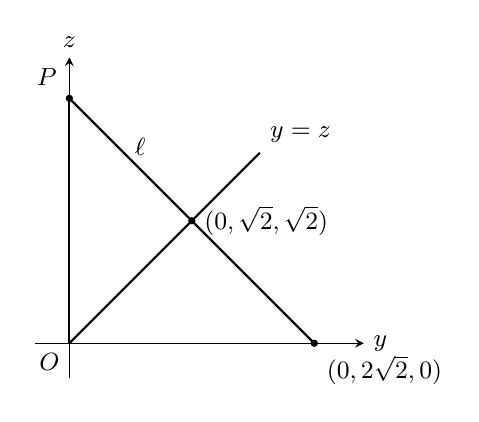
\begin{tikzpicture}[scale=1.1, >=stealth, every node/.style={font=\small}]
    % 平面 x=0 (yz平面) での断面図
    \draw[->] (-0.4,0) -- (3.4,0) node[right] {$y$};
    \draw[->] (0,-0.4) -- (0,3.3) node[above] {$z$};
    \node[below left] at (0,0) {$O$};

    % 直線 y=z （円 C を含む平面と x=0 平面の交線）
    \draw[thick] (0,0) -- (2.2,2.2) node[above right] {$y=z$};

    % 点光源 P と，円 C が x=0 平面を切る点 (0,\sqrt2,\sqrt2)
    \fill (0,2.828) circle (1.2pt) node[above left=1pt] {$P$};
    \fill (1.414,1.414) circle (1.2pt) node[right=1pt] {$(0,\sqrt{2},\sqrt{2})$};
    \fill (2.828,0) circle (1.2pt) node[below right=1pt] {$(0,2\sqrt{2},0)$};

    % 視線 (P からそれぞれの点を通り z=0 まで)
    \draw[thick] (0,2.828) -- (0,0);
    \draw[thick] (0,2.828) -- (2.828,0);

    % 点Pから直線 y=z への距離 \ell
    \draw[dashed] (0,2.828) -- (1.414,1.414) node[midway, above right=-2pt] {$\ell$};
  \end{tikzpicture}
  \caption{平面 $x=0$（$yz$ 平面）による切断面．円 $C$ はこの平面を点 $O$ と $(0,\sqrt{2},\sqrt{2})$ で切り，$P$ から直線 $y=z$ への距離 $\ell$ が (2) で用いる円錐の高さになる}
\end{figure}

点光源のある点を$P$とする．影$S$の境界の曲線を$C'$とし，$C'$上の点を$Q(X,Y,0)$とする．
題意から，$C$の中心は
$R\left(0,\dfrac{\sqrt{2}}{2},\dfrac{\sqrt{2}}{2}\right)$であり，また$C$は平面$y=z$にあるから，
$C$の外周$D$上の点$E$の満たす式は
\begin{align}
  D:
  \begin{cases}
    y=z \\
    x^2+\left(y-\dfrac{\sqrt{2}}{2}\right)^2 + \left(z-\dfrac{\sqrt{2}}{2}\right)^2 = 1
  \end{cases} \label{eq:1}
\end{align}
となる．$Q$の条件は，直線$PQ$が$D$と交わることである．直線$PQ$はパラメータを用いて
\begin{align}
  \begin{pmatrix}x\\y\\z
  \end{pmatrix}=
  \begin{pmatrix}0\\0\\2\sqrt{2}
  \end{pmatrix}+t
  \begin{pmatrix}X\\Y\\-2\sqrt{2}
  \end{pmatrix} \label{eq:2}
\end{align}
と表せるから，これが\cref{eq:1}を満たす$t$が存在すれば良い．
\cref{eq:2}を\cref{eq:1}に代入して
\begin{align}
  &
  \begin{cases}
    tY=2\sqrt{2}(1-t)  \\
    (tX)^2+\left(tY-\dfrac{\sqrt{2}}{2}\right)^2+\left(2\sqrt{2}(1-t)-\dfrac{\sqrt{2}}{2}\right)^2=1　
  \end{cases}
  &
  \begin{cases}
    tY=2\sqrt{2}(1-t)  \\
    (tX)^2+2\left(tY-\dfrac{\sqrt{2}}{2}\right)^2=1　
  \end{cases} \label{eq:3}
\end{align}
$Y \ge 0$に注意して，第一式から
\begin{align}
  t = \dfrac{2\sqrt{2}}{Y+2\sqrt{2}}
\end{align}
だから，第二式に代入してもとめる$C'$の方程式は
\begin{align}
  &\dfrac{8X^2}{(Y+2\sqrt{2})^2}+2\left(\dfrac{2\sqrt{2}Y}{Y+2\sqrt{2}}-\dfrac{\sqrt{2}}{2}\right)^2=1 \\
  \therefore&8X^2+2\left(\dfrac{3\sqrt{2}}{2}Y-2\right)^2=(Y+2\sqrt{2})^2 \\
  \therefore&X^2+(Y-\sqrt{2})^2=2\cdots\text{(答)}
\end{align}
である．

\subparagraph{(2)}
求める体積$V$とすれば，
\begin{align}
  V=(\text{円錐P-C'})-(\text{円錐P-C}) \label{eq:4}
\end{align}
である．円錐P-C'は(1)より底面積$\pi(\sqrt{2})=2\pi$，高さ$2\sqrt{2}$の円錐で，この体積$V_1$として
\begin{align}
  V_1=\dfrac{1}{3}(2\sqrt{2})(2\pi)=\dfrac{4\sqrt{2}}{3}\pi  \label{eq:5}
\end{align}
となる．

次に円錐P-Cについて，この高さは平面$y=z$と点$P$の距離$\ell$に等しく，点と直線の距離の公式から
\begin{align}
  \ell = \dfrac{2\sqrt{2}}{1+1} = 2
\end{align}
であり，底面積は半径$1$の円のそれ$\pi$である．故に体積$V_2$として
\begin{align}
  V_2=\dfrac{2}{3}\pi \label{eq:6}
\end{align}
である．
\cref{eq:5,eq:6}を\cref{eq:4}に代入して
\begin{align}
  V=\dfrac{2}{3}(2\sqrt{2}-1)\pi\cdots\text{(答)}
\end{align}
である．
\newpage
\end{document}
